\documentclass[a4paper,12pt]{article}
\usepackage[russian]{babel}
\usepackage[T2A]{fontenc}
\usepackage[utf8]{inputenc}
\usepackage{geometry}
\usepackage{amsmath}
\usepackage{graphicx}
\usepackage{cancel}
\usepackage{float} 
\usepackage{xcolor}
\usepackage{array}
\usepackage{caption}
\usepackage{booktabs}
\usepackage{amssymb}
\usepackage{subcaption}
\usepackage{pgfplots}
\pgfplotsset{compat=1.18}
\usetikzlibrary{arrows.meta, matrix}
\usepackage{capt-of}
\usepackage{multirow}
\usepackage[siunitx]{circuitikz}
\usepackage[bottom]{footmisc}
\usepackage{tcolorbox}
\usepackage{nicematrix}
\usepackage{tikz}
\usetikzlibrary{positioning, arrows.meta}

% --- hyperref ОДИН РАЗ ---
\usepackage{hyperref}
\hypersetup{linktoc=page}
\hypersetup{
	colorlinks=true,
	linkcolor=red,
	citecolor=red,
	urlcolor=red,
	filecolor=red,
}

% --- Содержание ---
\usepackage{tocloft}
\usepackage{etoolbox}
\usepackage{hyperref}
\hypersetup{
	colorlinks=true,
	linkcolor=red,
	citecolor=red,
	urlcolor=red,
}

% Патчим \tableofcontents: текст строк — без ссылок и чёрный
% Это делается через замену \contentsline внутри TOC
\preto\tableofcontents{%
	\begingroup
	% Переопределяем contentsline так, чтобы текст был чёрным без ссылки,
	% а номер страницы — красной ссылкой
	\renewcommand{\contentsline}[4]{%
		\ifnum\pdfstrcmp{##1}{section}=0
		\vskip 4pt{\normalfont\color{black}##2}\nobreak\hfill
		{\normalfont\color{red}\hyperlink{##4}{##3}}\par
		\else\ifnum\pdfstrcmp{##1}{subsection}=0
		\vskip 2pt\hspace{1.5em}{\normalfont\color{black}##2}\nobreak\hfill
		{\normalfont\color{red}\hyperlink{##4}{##3}}\par
		\else
		\vskip 1pt\hspace{3em}{\normalfont\color{black}##2}\nobreak\hfill
		{\normalfont\color{red}\hyperlink{##4}{##3}}\par
		\fi\fi
	}%
}
\appto\tableofcontents{\endgroup}

% tocloft — только для отступов, без переопределения шрифтов
\usepackage{tocloft}

% --- Листинги ---
\usepackage{listings}

\definecolor{codebg}{RGB}{250,250,252}
\definecolor{linenumcolor}{RGB}{150,150,170}
\definecolor{mathblue}{RGB}{30,100,200}
\definecolor{mathorange}{RGB}{200,100,20}
\definecolor{matlabblue}{RGB}{0,0,200}
\definecolor{matlabgreen}{RGB}{30,130,30}
\definecolor{matlaborange}{RGB}{200,80,0}


\lstdefinestyle{matlab}{
	language=Matlab,
	basicstyle=\ttfamily\small,
	keywordstyle=\color{matlabblue}\bfseries,
	commentstyle=\color{matlabgreen}\itshape,
	stringstyle=\color{matlaborange},
	numberstyle=\tiny\color{linenumcolor},
	numbers=left,
	numbersep=10pt,
	backgroundcolor=\color{codebg},
	frame=single,
	frameround=tttt,
	framesep=4pt,
	rulecolor=\color{matlabblue!30},
	breaklines=true,
	tabsize=4,
	showstringspaces=false,
	captionpos=b,
	xleftmargin=15pt,
	xrightmargin=5pt,
	escapeinside={\%*}{*)},
	morekeywords={cvx_begin,cvx_end,sdp,variable,minimize,maximize},
}

\lstset{style=matlab}

\renewcommand{\lstlistingname}{Листинг}
\DeclareCaptionFormat{redlisting}{#1\textcolor{red}{#2}#3}
\captionsetup[lstlisting]{format=redlisting}

\geometry{left=1.5cm, right=2cm, bottom=2cm, top=2cm}
\captionsetup[figure]{name=Рисунок}
\captionsetup[table]{name=Таблица}
\captionsetup{labelsep=endash}

\newcommand{\figwidth}{0.6\textwidth}

\begin{document}
	
	\begin{titlepage}
		\centering
		
		\vspace*{0.5cm}
		{\small
			Министерство науки и высшего образования Российской Федерации\\[2pt]
			Федеральное государственное автономное образовательное учреждение\\
			высшего образования\\[2pt]
			\textbf{«Национальный исследовательский университет ИТМО»}\\
		}
		
		\vspace{0.8cm}
		\hrule height 0.8pt
		\vspace{0.3cm}
		
		{\large Факультет систем управления и робототехники}
		
		\vspace{0.3cm}
		\hrule height 0.4pt
		\vspace{2.5cm}
		
		{\Huge\bfseries ОТЧЁТ}\\[0.4cm]
		{\LARGE\bfseries о лабораторной работе}\\[0.8cm]
		
		\begin{tcolorbox}[
			colback=gray!4,
			colframe=gray!10,
			boxrule=0.8pt,
			arc=4pt,
			left=12pt, right=12pt, top=8pt, bottom=8pt
			]
			\centering
			{\large По дисциплине:\\[4pt]}
			{\large\bfseries «Теория автоматического управления»}\\[10pt]
			{\large Тема:\\[4pt]}
			{\large\bfseries «Линейно-квадратичные радости»} \\[10pt]
			{\large Поток: 1.1.3 \( \) Вариант: 25}
		\end{tcolorbox}
		
		\vspace{3cm}
		
		\begin{minipage}{0.45\textwidth}
			\raggedright
			{\large\bfseries Студент:}\\[4pt]
			Охрименко Е.\,Д.\\
		\end{minipage}
		\hfill
		\begin{minipage}{0.45\textwidth}
			\raggedleft
			{\large\bfseries Преподаватель:}\\[4pt]
			Пашенко А.\,В.\\
		\end{minipage}
		
		\vfill
		\vspace{0.4cm}
		{\large Санкт-Петербург, 2026}
	\end{titlepage}
	
	\newpage
	\tableofcontents
	
	\newpage \section{Исследование LQR}\label{sec:1}
	
	В соответствии с вариантом рассмотрю систему:
	
	\begin{equation}
		\begin{cases}
			\dot{x} = Ax + Bu \\
		\end{cases}
		\qquad
		x(0) = \begin{bmatrix} 1 & 1 & 1 \end{bmatrix}^T
		\label{sys}
	\end{equation}
	
	где:
	
	\[
	A = \begin{bmatrix} 
		8 & 1 & 11 \\ 
		4 & 0 & 4 \\ 
		-4 & -3 & -7 
	\end{bmatrix} \quad
	B = \begin{bmatrix} -1 \\ -3 \\ 3 \end{bmatrix} 
	\]
	
	
	Требуется:
	\begin{enumerate}
		\item Проверить систему $\dot{x} = Ax + Bu$ на стабилизируемость.
		
		\item Построить схему моделирования с регулятором $u = Kx$.
		
		\item Выбрать $Q \succ 0$, $R \succ 0$, $\alpha > 0$ и сформировать четыре пары $(Q,R)$: $(Q,R)$, $(\alpha Q,R)$, $(Q,\alpha R)$, $(\alpha Q,\alpha R^*)$.
		
		\item Для каждой пары $(Q,R)$ решить уравнение Риккати 
		\[
		A^T P + PA + Q - PBR^{-1}B^T P = 0,
		\]
		найти $K = R^{-1}B^T P$, вычислить $J_{min} = x_0^T P x_0$, выполнить моделирование и построить графики $u(t)$, $x(t)$, $J_{exp}(t)$. Сопоставить $J_{exp}(t)$ с $J_{min}$.
		
		\item Сравнить результаты для разных $(Q,R)$, сделать выводы.
	\end{enumerate}
	
	\hrule \newpage
	
	
	
	
	\subsection{Стабилизируемость системы}
	
	Для начала найду собственные числа матрицы $A$, решив характеристическое уравнение $\det(\lambda I - A) = 0$:
	
	\[
	\det(\lambda I - A) =
	\det\begin{bmatrix}
		\lambda - 8 & -1 & -11 \\
		-4 & \lambda & -4 \\
		4 & 3 & \lambda + 7
	\end{bmatrix} = 0
	\]
	
	Получаю характеристическое уравнение и следующие собственные числа:
	\[
	\lambda^3 - \lambda^2 - 4\lambda + 24 = 0
	\qquad \Longrightarrow \qquad
	\lambda_1 = -3, \quad \lambda_{2,3} = 2 \pm 2i
	\]
	
	Для оценки управляемости каждого собственного числа, построю Жорданову вещественную форму (листинг~\ref{lst:jordan1}). Тогда система в Жордановом базисе будет иметь вид:
	
	\[
	\dot{\hat{x}} = 
	\begin{bNiceMatrix}[create-medium-nodes, left-margin=4pt, right-margin=4pt]
		-3 & 0 & 0 \\
		0 & 2 & -2 \\
		0 & 2 & 2 \\
		\CodeAfter
		\tikz \draw[red!80!black, rounded corners=2pt, line width=0.7pt, opacity=0.4] 
		([xshift=-2pt, yshift=2pt]1-1-medium.north west) rectangle 
		([xshift=2pt, yshift=-2pt]1-1-medium.south east);
		\tikz \draw[green!40!black, rounded corners=4pt, line width=0.7pt, opacity=0.4] 
		([xshift=-2pt, yshift=2pt]2-2-medium.north west) rectangle 
		([xshift=2pt, yshift=-2pt]3-3-medium.south east);
	\end{bNiceMatrix}
	\hat{x}  + 
	\begin{bNiceMatrix}[create-medium-nodes, left-margin=4pt, right-margin=4pt]
		0 \\ 2.12 \\ 4.95 \\
		\CodeAfter
		\tikz \draw[red!80!black, rounded corners=2pt, line width=0.7pt, opacity=0.4]
		([xshift=-2pt, yshift=2pt]1-1-medium.north west) rectangle 
		([xshift=2pt, yshift=-2pt]1-1-medium.south east);
		\tikz \draw[green!40!black, rounded corners=4pt, line width=0.7pt, opacity=0.4]
		([xshift=-2pt, yshift=2pt]2-1-medium.north west) rectangle 
		([xshift=2pt, yshift=-2pt]3-1-medium.south east);
	\end{bNiceMatrix}
	u
	\]
	
	Собственное число \(\lambda_1 = -3\) неуправляемо, так как ему соответствует элемент \(0\) в матрице \(\hat{B}\). Собственные числа $\lambda_{2,3} = 2 \pm 2i$ управляемы, так как 
	последняя строка соответствующего блока в матрице $\hat{B}$ ненулевая.
	
	Получается, что система в целом не является полностью управляемой.
	
	Неуправляемое собственное число \(\lambda_1 = -3\) лежит в левой комплексной полуплоскости, а значит система стабилизируема.
	
	\subsection{Структурная схема системы}
	
	Построю схему моделирования системы, замкнутой регулятором \(u=-K x\):
	
	
	\begin{figure}[H]
		\centering
		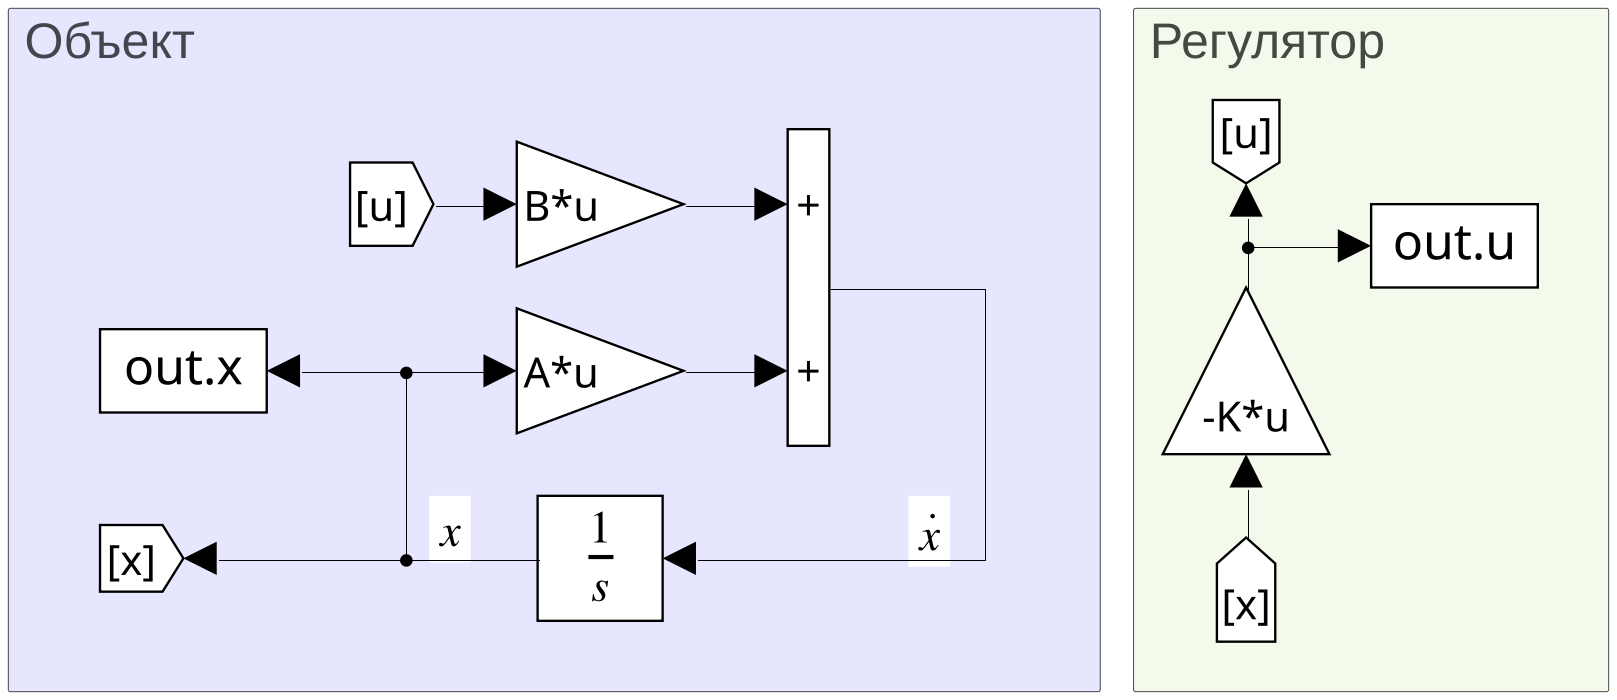
\includegraphics[width=\figwidth]{../../report/images/task1/closed.png}
		\caption{Структурная схема замкнутой системы}
	\end{figure}
	
	
	\subsection{Выбор параметров $(Q, R)$}
	
	Задам матрицы $Q_0 \succ 0$, $R_0 \succ 0$, параметр $\alpha > 0$:
	
	\[
	Q_0 = I = 
	\begin{bmatrix}
		1 & 0 & 0 \\
		0 & 1 & 0 \\
		0 & 0 & 1
	\end{bmatrix}, \quad
	R_0 = 1, \quad
	\alpha = 5.
	\]
	
	Сформирую наборы:
	
	\begin{enumerate}
		\item $(Q, R) = (Q_0, R_0) = 
		\left(
		\begin{bmatrix}
			1 & 0 & 0 \\
			0 & 1 & 0 \\
			0 & 0 & 1
		\end{bmatrix}, 1
		\right)$
		
		\item $(Q, R) = (\alpha Q_0, R_0) = 
		\left(
		\begin{bmatrix}
			5 & 0 & 0 \\
			0 & 5 & 0 \\
			0 & 0 & 5
		\end{bmatrix}, 1
		\right)$
		
		\item $(Q, R) = (Q_0, \alpha R_0) = 
		\left(
		\begin{bmatrix}
			1 & 0 & 0 \\
			0 & 1 & 0 \\
			0 & 0 & 1
		\end{bmatrix}, 5
		\right)$
		
		\item $(Q, R) = (\alpha Q_0, \alpha R_0) = 
		\left(
		\begin{bmatrix}
			5 & 0 & 0 \\
			0 & 5 & 0 \\
			0 & 0 & 5
		\end{bmatrix}, 5
		\right)$
	\end{enumerate}
	
	
	\subsection{Синтез LQR-регуляторов}
	
	Для каждой из пар значений матриц $(Q, R)$ я синтезирую регулятор, минимизирующий функционал качества:
	
	\[
	J = \int_{0}^{\infty} \left( x(t)^T Q x(t) + u(t)^T R u(t) \right) dt,
	\]
	
	где $Q$ --- штраф на вектор состояния, а $R$ --- штраф на управление. Синтез выполняется путем решения матричного уравнения Риккати при $\nu = 1$:
	
	\[
	A^T P + P A + Q - \nu P B R^{-1} B^T P = 0, \qquad K = R^{-1} B^T P.
	\]
	
	Затем я вычисляю соответствующее минимальное значение функционала качества:
	
	\[
	J_{min} = x_0^T P x_0.
	\]
	
	
	
	
	Результаты для четырёх наборов $(Q,R)$ сведены в таблицу \ref{tab:lqr_results} (листинг~\ref{lst:LQR1}):
	
	\begin{table}[H]
		\centering
		\caption{Результаты синтеза LQR-регуляторов}
		\label{tab:lqr_results}
		\renewcommand{\arraystretch}{1.3}
		\begin{tabular}{@{}lcc@{}}
			\toprule
			\textbf{Набор} & \textbf{\(K\)} & \textbf{\(J_{min}\)} \\
			\midrule
			\((Q_0, R_0)\) & \([6.4000, \ -0.7945, \ 5.9633]\) & \(15.4517\) \\
			\((\alpha Q_0, R_0)\) & \([11.0686, \ -0.5843, \ 9.8909]\) & \(40.3691\) \\
			\((Q_0, \alpha R_0)\) & \([4.1727, \ -0.8479, \ 4.0290]\) & \(37.9133\) \\
			\((\alpha Q_0, \alpha R_0)\) & \([6.4000, \ -0.7945, \ 5.9633]\) & \(77.2586\) \\
			\bottomrule
		\end{tabular}
	\end{table}
	
Матрицы $P$ для каждого набора:

\[
\begin{aligned}
	P_{(Q_0,R_0)} &= 
	\begin{bmatrix}
		4.28 & 0.07 & 3.63 \\
		0.07 & 0.33 & 0.08 \\
		3.63 & 0.08 & 3.28
	\end{bmatrix} &
	P_{(\alpha Q_0,R_0)} &= 
	\begin{bmatrix}
		11.03 & 1.04 & 8.41 \\
		1.04 & 0.97 & 1.12 \\
		8.41 & 1.12 & 7.22
	\end{bmatrix} \\[1.2cm]
\end{aligned}
\]

\[\begin{aligned}
	P_{(Q_0,\alpha R_0)} &= \begin{bmatrix}
		10.63 & -0.68 & 9.82 \\
		-0.68 & 0.98 & -0.66 \\
		9.82 & -0.66 & 9.33
	\end{bmatrix} &
	P_{(\alpha Q_0,\alpha R_0)} &= 
	\begin{bmatrix}
		21.38 & 0.35 & 18.14 \\
		0.35 & 1.63 & 0.42 \\
		18.14 & 0.42 & 16.41
	\end{bmatrix}
\end{aligned}
\]
	
	\subsection{Моделирование}
	
	Построю график \(J_{exp}(t)\). Пунктирными линиями обозначу соответственно вычисленное значение функционала качества \(J_{min}\).
	
	
	
	\begin{figure}[H]
		\centering
		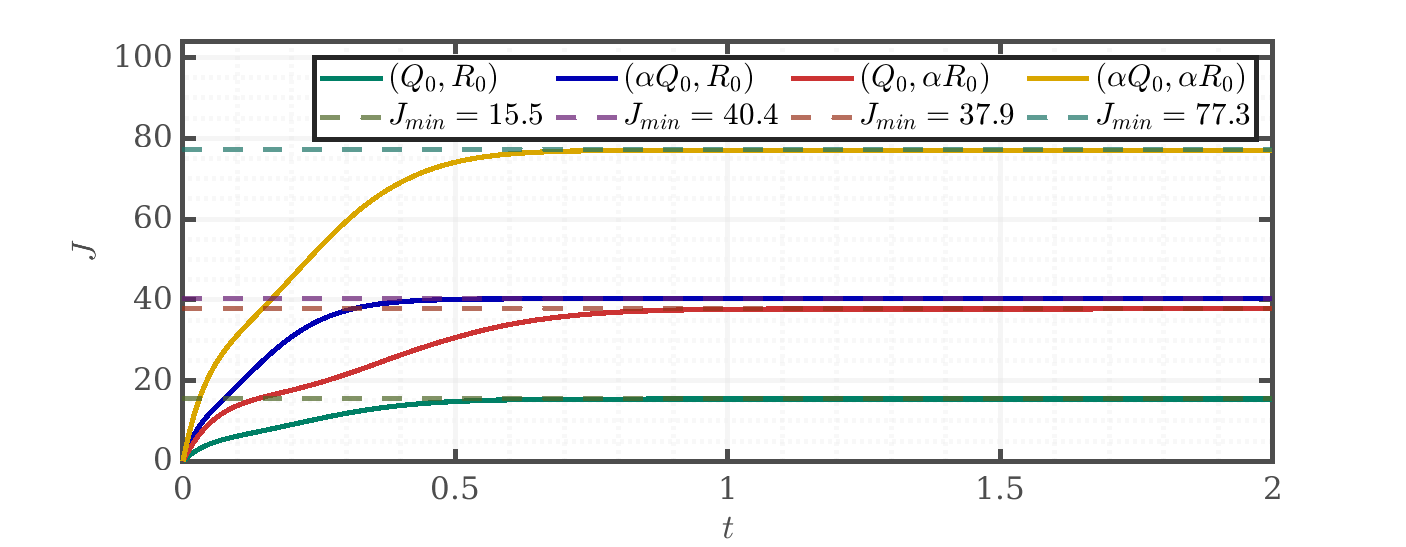
\includegraphics[width=\figwidth]{../../report/images/task1/J.png}
		\caption{Функционалы качества}
	\end{figure}
	
	Построю графики управления для 4-x наборов на одном рисунке.
	
	\begin{figure}[H]
		\centering
		
\includegraphics[width=\figwidth]{../../report/images/task1/u.png}
		\caption{Управления}
	\end{figure}
	
	Графики векторов состояний приведены ниже.
	
	\begin{figure}[H]
		\centering
		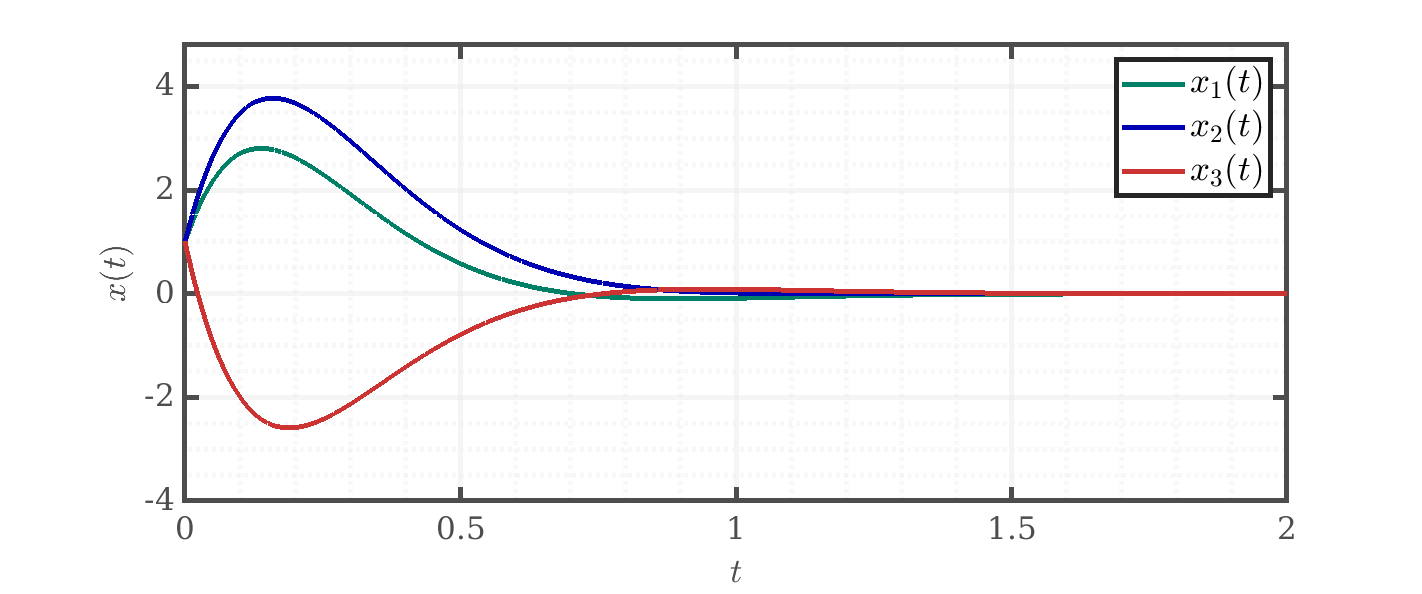
\includegraphics[width=\figwidth]{../../report/images/task1/x_1.png}
		\caption{Состояние системы $x(t)$ для набора 1: $(Q_0, R_0)$}
	\end{figure}
	
	\begin{figure}[H]
		\centering
		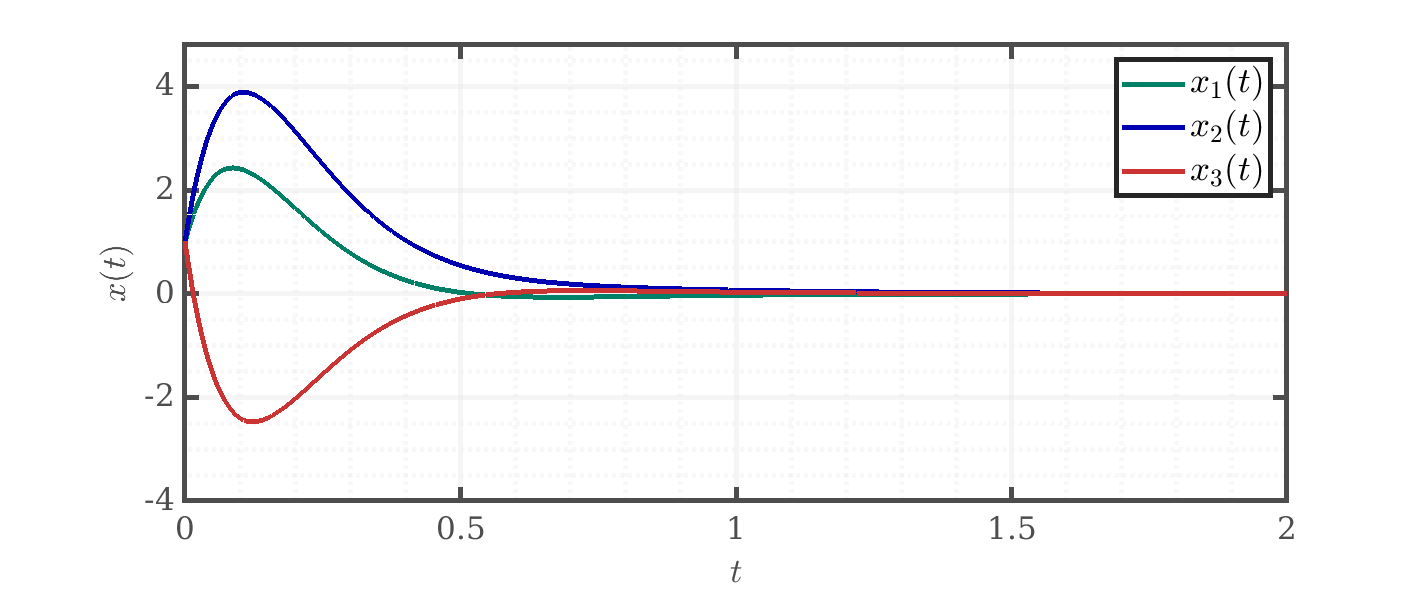
\includegraphics[width=\figwidth]{../../report/images/task1/x_2.png}
		\caption{Состояние системы $x(t)$ для набора 2: $(\alpha Q_0, R_0)$}
	\end{figure}
	
	\begin{figure}[H]
		\centering
		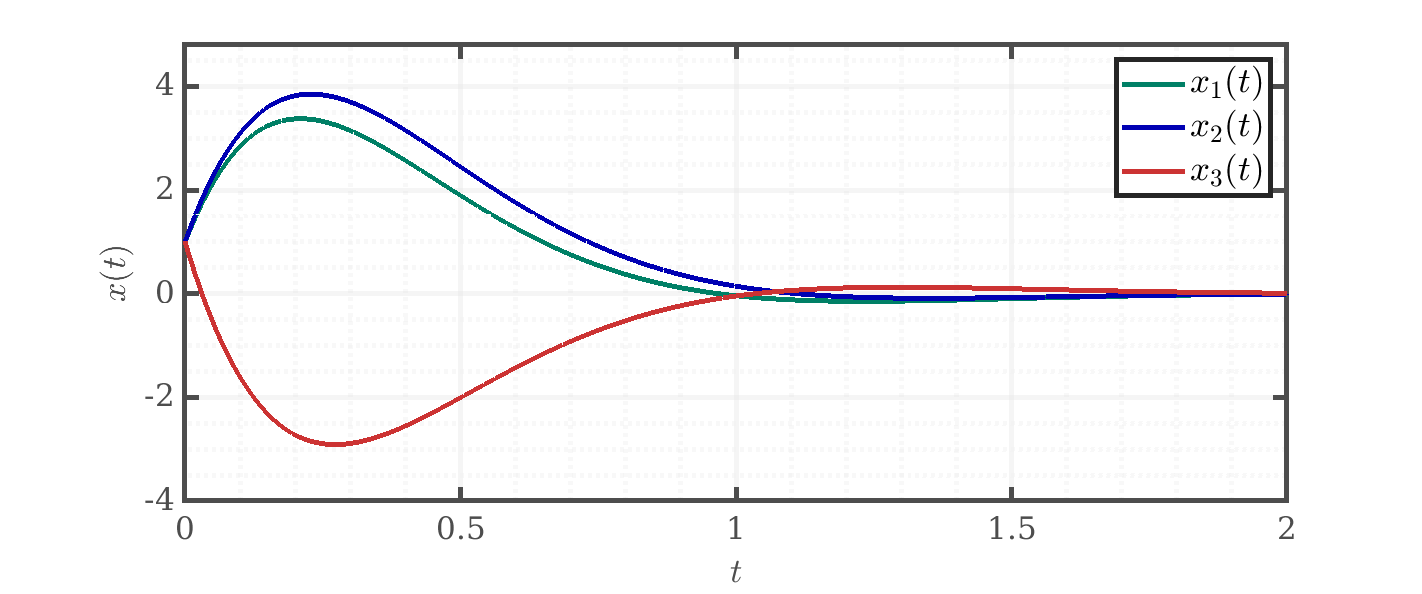
\includegraphics[width=\figwidth]{../../report/images/task1/x_3.png}
		\caption{Состояние системы $x(t)$ для набора 3: $(Q_0, \alpha R_0)$}
	\end{figure}
	
	\begin{figure}[H]
		\centering
		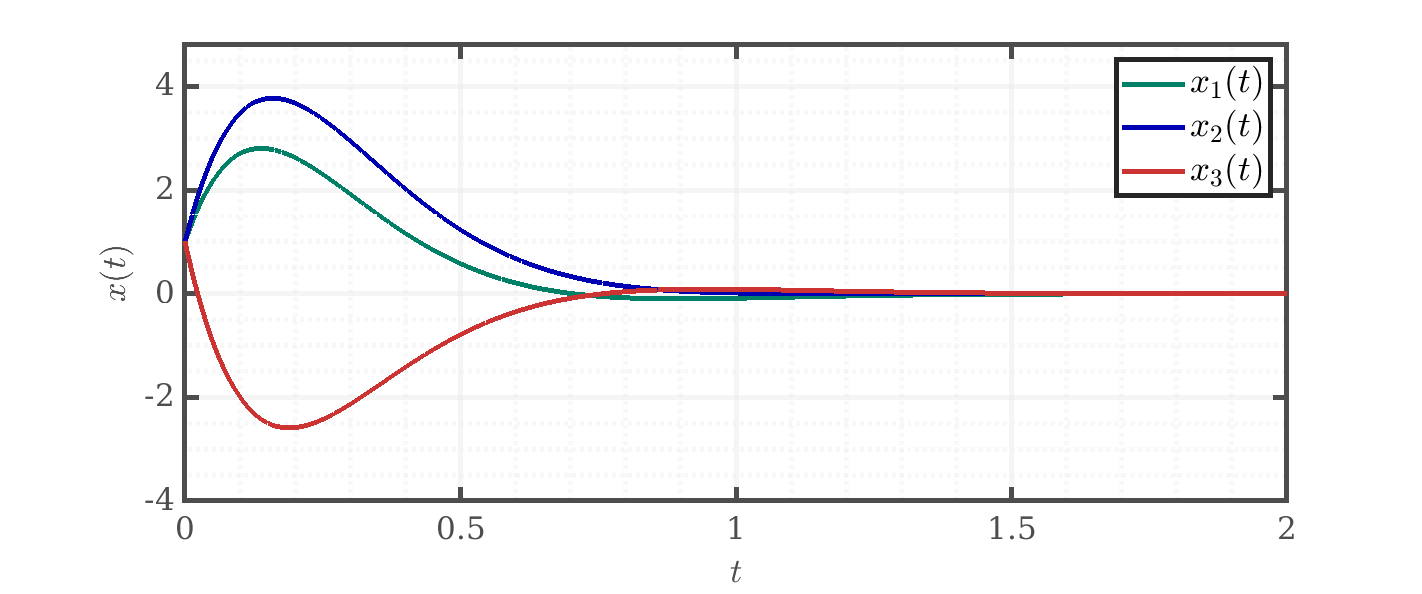
\includegraphics[width=\figwidth]{../../report/images/task1/x_4.png}
		\caption{Состояние системы $x(t)$ для набора 4: $(\alpha Q_0, \alpha R_0)$}
	\end{figure}
	
	\newpage
	\subsection{Выводы}
	
	В ходе работы синтезирован LQR-регулятор для системы третьего порядка.
	
	\begin{enumerate}
		\item Система стабилизируема: неуправляемое собственное число $\lambda = -3$ лежит в левой полуплоскости.
		
		\item Увеличение $Q$ (набор 2) усиливает управление, ускоряет затухание переходных процессов, увеличивает $J_{min}$.
		
		\item Увеличение $R$ (набор 3) ослабляет управление, замедляет переходные процессы, увеличивает $J_{min}$.
		
		\item Одновременное масштабирование $Q$ и $R$ (набор 4) не меняет $K$, а $J_{min}$ масштабируется пропорционально $\alpha$.
		
		\item $J_{exp}(t)$ сходится к $J_{min}$ во всех экспериментах, что подтверждает корректность синтеза.
	\end{enumerate}
	
	Таким образом, выбор весовых матриц $Q$ и $R$ определяет, насколько быстро затухают переходные процессы и насколько интенсивно управление.
	
	
	
	
	\newpage \section{Исследование LQE и фильтра Калмана}\label{sec:2}

В соответствии с вариантом рассмотрю систему:

\begin{equation}
	\begin{cases}
		\dot{x} = Ax + f \\
		y = Cx + \xi
	\end{cases}
	\qquad
	x(0) = \begin{bmatrix} 1 & 1 & 1 & 1 \end{bmatrix}^T
	\label{sys2}
\end{equation}

где:

\[
A = \begin{bmatrix} 
	-40 & 16 & 9 & 7 \\ 
	-64 & 25 & 14 & 12 \\ 
	-26 & 11 & 7 & 3 \\ 
	-48 & 18 & 14 & 8 \\ 

\end{bmatrix} \quad
C^T = \begin{bmatrix} -3 \\ 2 \\ -2 \\ 1 \\  \end{bmatrix} 
\]


Требуется:
\begin{enumerate}
	\item Проверить систему на обнаруживаемость.
	
	\item Построить схему моделирования системы с наблюдателем состояния.
	
	\item Выбрать $Q \succ 0$, $R \succ 0$, $\alpha > 0$ и сформировать четыре пары $(Q,R)$: $(Q,R)$, $(\alpha Q,R)$, $(Q,\alpha R)$, $(\alpha Q,\alpha R)$. При необходимости предложить дополнительный набор для полного подавления возмущений.
	
	\item Для каждой пары $(Q,R)$ решить уравнение Риккати
	\[
	AP + PA^T + Q - PC^T R^{-1} C P = 0,
	\]
	найти $L = PC^T R^{-1}$, выполнить моделирование с нулевыми начальными условиями наблюдателя $\hat{x}(0) = 0$ и построить графики $x(t)$, $\hat{x}(t)$ и ошибки $e(t) = x(t) - \hat{x}(t)$.
	
	\item Сравнить результаты для разных $(Q,R)$, сделать выводы.
\end{enumerate}

\hrule \newpage	
	
	
\subsection{Проверка обнаруживаемости}

Матрица наблюдаемости (листинг~\ref{lst:obsv}):

\[
\mathcal{O} = 
\begin{bmatrix}
	C \\ CA \\ CA^2 \\ CA^3
\end{bmatrix}
=
\begin{bmatrix}
	-3 & 2 & -2 & 1 \\
	-4 & -2 & 1 & 5 \\
	22 & -13 & 13 & -9 \\
	46 & 8 & -19 & -35
\end{bmatrix}
\]

\[
\text{rank}(\mathcal{O}) = 4 = \text{rank}(A)
\]

Так как система полностью наблюдаема, она является обнаруживаемой. Синтез наблюдателя возможен.	
	


\subsection{Структурная схема системы}

Построю схему моделирования системы. Объект управления описывается уравнениями:

\[
\begin{cases}
	\dot{x} = Ax + f \\
	y = Cx + \xi
\end{cases}
\]

Наблюдатель состояния имеет структуру:

\[
\dot{\hat{x}} = (A-L C)\hat{x} +L y \qquad \hat{x}(0) =\begin{bmatrix} 0 & 0 & 0 & 0 \end{bmatrix}^T
\]

\begin{figure}[H]
	\centering
	
\includegraphics[width=0.8\textwidth]{../../report/images/task2/closed_observer.png}
	\caption{Схема моделирования системы с наблюдателем состояния}
\end{figure}

	
	\subsection{Выбор параметров $(Q, R)$}

Задам матрицы $Q_0 \succ 0$, $R_0 \succ 0$, параметр $\alpha > 0$:

\[
Q_0 = I = 
\begin{bmatrix}
	1 & 0 & 0 \\
	0 & 1 & 0 \\
	0 & 0 & 1
\end{bmatrix}, \quad
R_0 = 1, \quad
\alpha = 5.
\]

Сформирую наборы:

\begin{enumerate}
	\item $(Q, R) = (Q_0, R_0) = 
	\left(
	\begin{bmatrix}
		1 & 0 & 0 \\
		0 & 1 & 0 \\
		0 & 0 & 1
	\end{bmatrix}, 1
	\right)$
	
	\item $(Q, R) = (\alpha Q_0, R_0) = 
	\left(
	\begin{bmatrix}
		5 & 0 & 0 \\
		0 & 5 & 0 \\
		0 & 0 & 5
	\end{bmatrix}, 1
	\right)$
	
	\item $(Q, R) = (Q_0, \alpha R_0) = 
	\left(
	\begin{bmatrix}
		1 & 0 & 0 \\
		0 & 1 & 0 \\
		0 & 0 & 1
	\end{bmatrix}, 5
	\right)$
	
	\item $(Q, R) = (\alpha Q_0, \alpha R_0) = 
	\left(
	\begin{bmatrix}
		5 & 0 & 0 \\
		0 & 5 & 0 \\
		0 & 0 & 5
	\end{bmatrix}, 5
	\right)$
\end{enumerate}	
	
	
\subsection{Синтез наблюдателей LQE}

Для каждой из пар значений матриц $(Q, R)$ я синтезирую наблюдатель, минимизирующий критерий доверия:

\[
J = \int_{0}^{\infty} \left( f^T(t) Q^{-1} f(t) + \xi^T(t) R^{-1} \xi(t) \right) dt
\]

где $Q$ --- интенсивность шума процесса, а $R$ --- интенсивность шума измерения. Синтез выполняется путем решения матричного уравнения Риккати при $\nu = 1$ (листинг~\ref{lst:LQE2}):

\[
AP + PA^T + Q - \nu PC^T R^{-1} C P = 0 \qquad L = PC^T R^{-1}.
\]

Результаты для четырёх наборов $(Q,R)$ сведены в таблицу \ref{tab:lqe_results}:

\begin{table}[H]
	\centering
	\caption{Результаты синтеза наблюдателей LQE}
	\label{tab:lqe_results}
	\renewcommand{\arraystretch}{1.3}
	\begin{tabular}{@{}lc@{}}
		\toprule
		\textbf{Набор} & \textbf{\(L\)} \\
		\midrule
		\((Q_0, R_0)\) & \([-5.6331, \ -6.7056, \ -3.6304, \ -5.3790]^T\) \\
		\((\alpha Q_0, R_0)\) & \([-18.5024, \ -24.5390, \ -11.8335, \ -19.0512]^T\) \\
		\((Q_0, \alpha R_0)\) & \([-1.3945, \ -1.2265, \ -0.9807, \ -1.0964]^T\) \\
		\((\alpha Q_0, \alpha R_0)\) & \([-5.6331, \ -6.7056, \ -3.6304, \ -5.3790]^T\) \\
		\bottomrule
	\end{tabular}
\end{table}

Матрицы $P$ для каждого набора:

\[
\begin{aligned}
	P_{(Q_0,R_0)} &= 
	\begin{bmatrix}
		295.42 & 463.64 & 206.11 & 365.58 \\
		463.64 & 729.86 & 325.12 & 574.73 \\
		206.11 & 325.12 & 145.79 & 256.05 \\
		365.58 & 574.73 & 256.05 & 454.01
	\end{bmatrix} &
	P_{(\alpha Q_0,R_0)} &= 
	\begin{bmatrix}
		1348.70 & 2117.70 & 942.90 & 1678.00 \\
		2117.70 & 3333.40 & 1488.30 & 2638.40 \\
		942.90 & 1488.30 & 668.60 & 1177.60 \\
		1678.00 & 2638.40 & 1177.60 & 2093.50
	\end{bmatrix} \\[1.5cm]
	P_{(Q_0,\alpha R_0)} &= 
	\begin{bmatrix}
		370.12 & 581.83 & 257.47 & 454.66 \\
		581.83 & 918.19 & 406.58 & 716.14 \\
		257.47 & 406.58 & 181.59 & 317.53 \\
		454.66 & 716.14 & 317.53 & 561.27
	\end{bmatrix} &
	P_{(\alpha Q_0,\alpha R_0)} &= 
	\begin{bmatrix}
		1477.10 & 2318.20 & 1030.60 & 1827.90 \\
		2318.20 & 3649.30 & 1625.60 & 2873.70 \\
		1030.60 & 1625.60 & 729.00 & 1280.30 \\
		1827.90 & 2873.70 & 1280.30 & 2270.00
	\end{bmatrix}
\end{aligned}
\]
	
	
\subsection{Моделирование}

Для каждого из четырёх наборов матриц $(Q,R)$ выполнено компьютерное моделирование системы с наблюдателем состояния. Начальные условия наблюдателя заданы нулевыми:
\[
\hat{x}(0) = \begin{bmatrix} 0 & 0 & 0 & 0 \end{bmatrix}^T.
\]

Возмущения заданы в виде гармонических сигналов:

\[
f(t) = 
\begin{bmatrix}
	0.5 \sin(2t) \\
	0.5 \sin(2t) \\
	0.5 \sin(2t) \\
	0.5 \sin(2t)
\end{bmatrix} \qquad
\xi(t) = 0.1 \sin\left(5t + \frac{\pi}{4}\right)
\]

Графики ошибки наблюдения $e(t) = x(t) - \hat{x}(t)$ для всех наборов представлены ниже.

\begin{figure}[H]
	\centering
	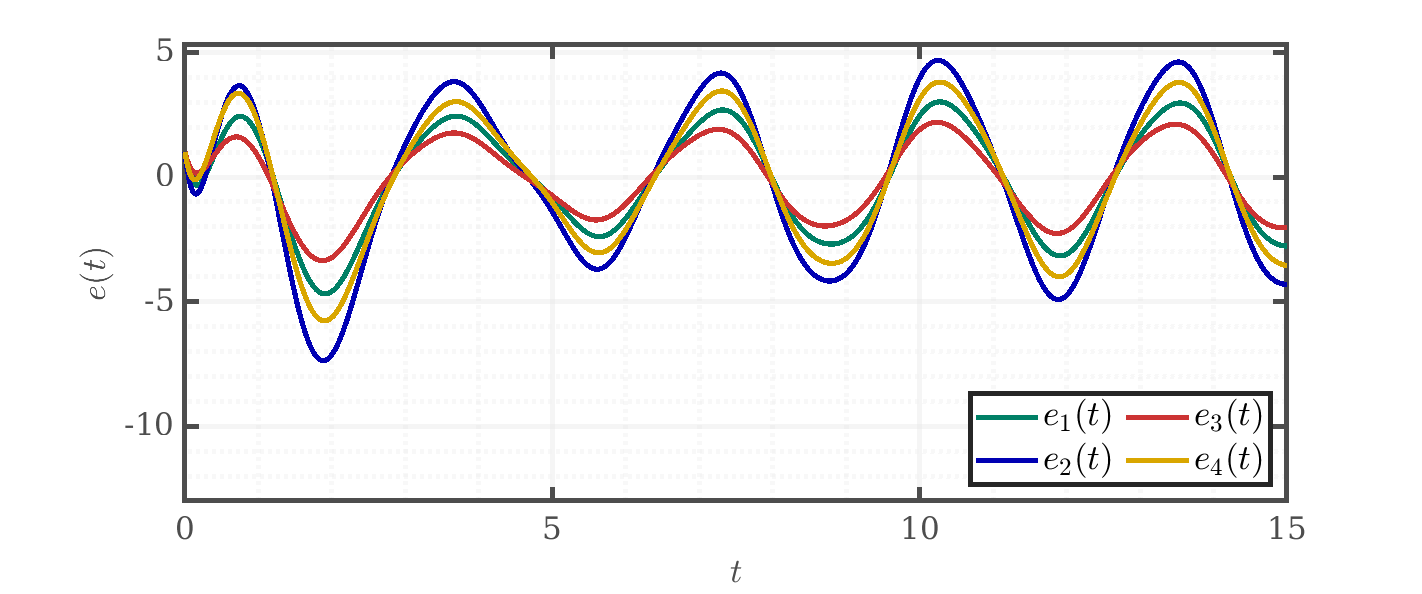
\includegraphics[width=\figwidth]{../../report/images/task2/e_1.png}
	\caption{Ошибка наблюдения для набора 1: $(Q_0, R_0)$}
\end{figure}

\begin{figure}[H]
	\centering
	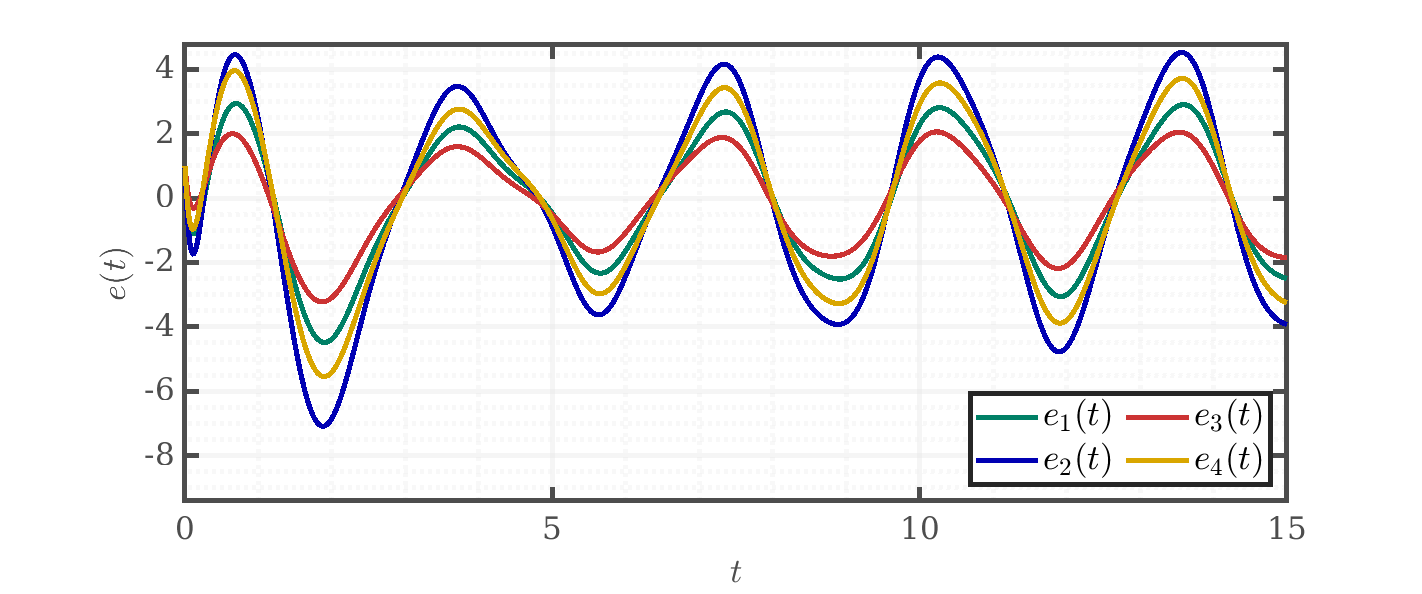
\includegraphics[width=\figwidth]{../../report/images/task2/e_2.png}
	\caption{Ошибка наблюдения для набора 2: $(\alpha Q_0, R_0)$}
\end{figure}

\begin{figure}[H]
	\centering
	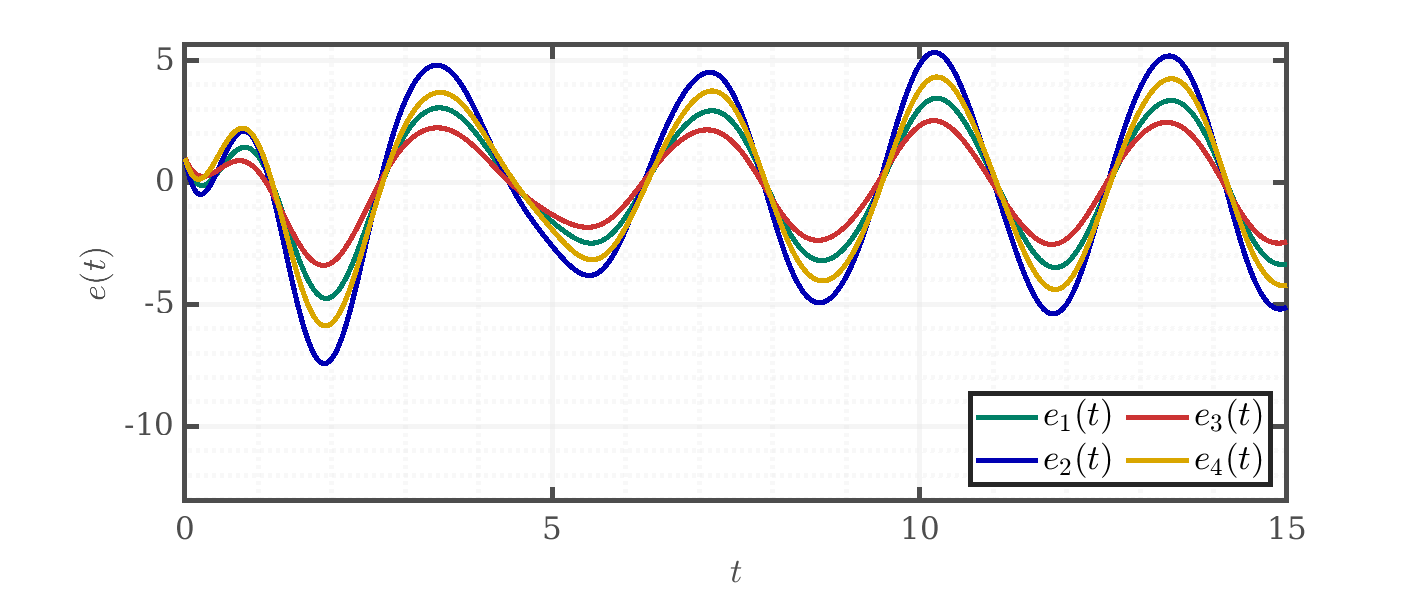
\includegraphics[width=\figwidth]{../../report/images/task2/e_3.png}
	\caption{Ошибка наблюдения для набора 3: $(Q_0, \alpha R_0)$}
\end{figure}

\begin{figure}[H]
	\centering
	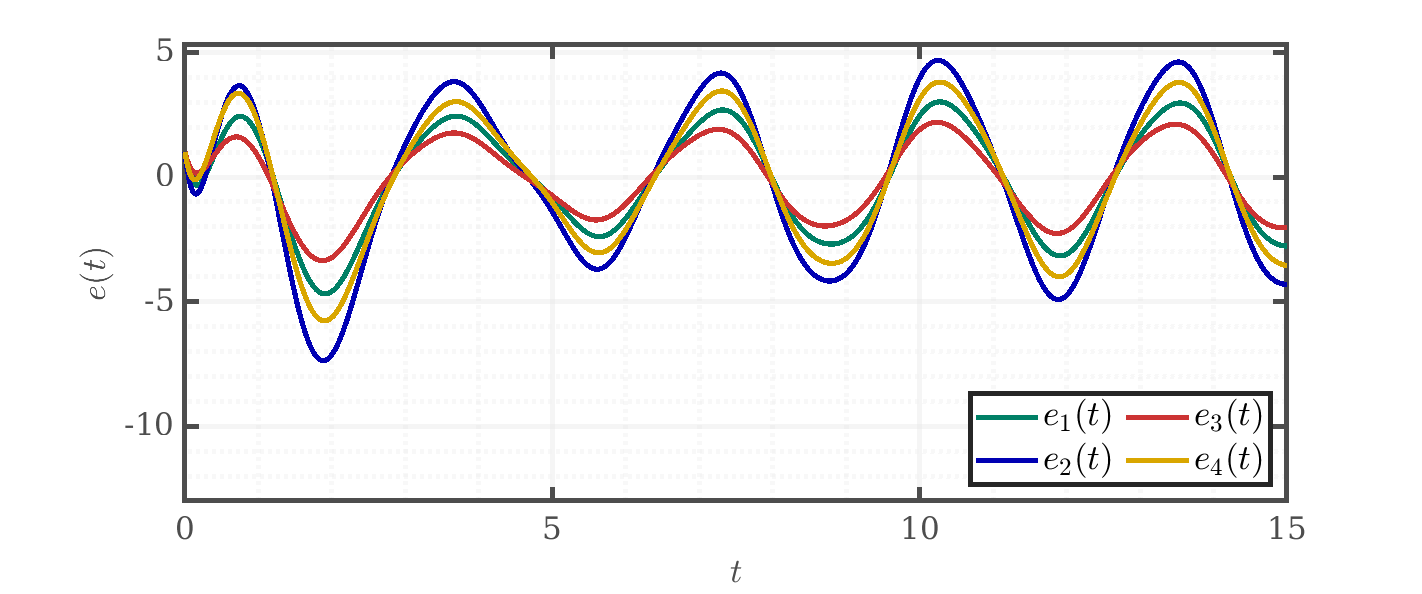
\includegraphics[width=\figwidth]{../../report/images/task2/e_4.png}
	\caption{Ошибка наблюдения для набора 4: $(\alpha Q_0, \alpha R_0)$}
\end{figure}

Сравнительные графики истинного состояния $x(t)$ и его оценки $\hat{x}(t)$ для каждого набора приведены ниже.

\begin{figure}[H]
	\centering
	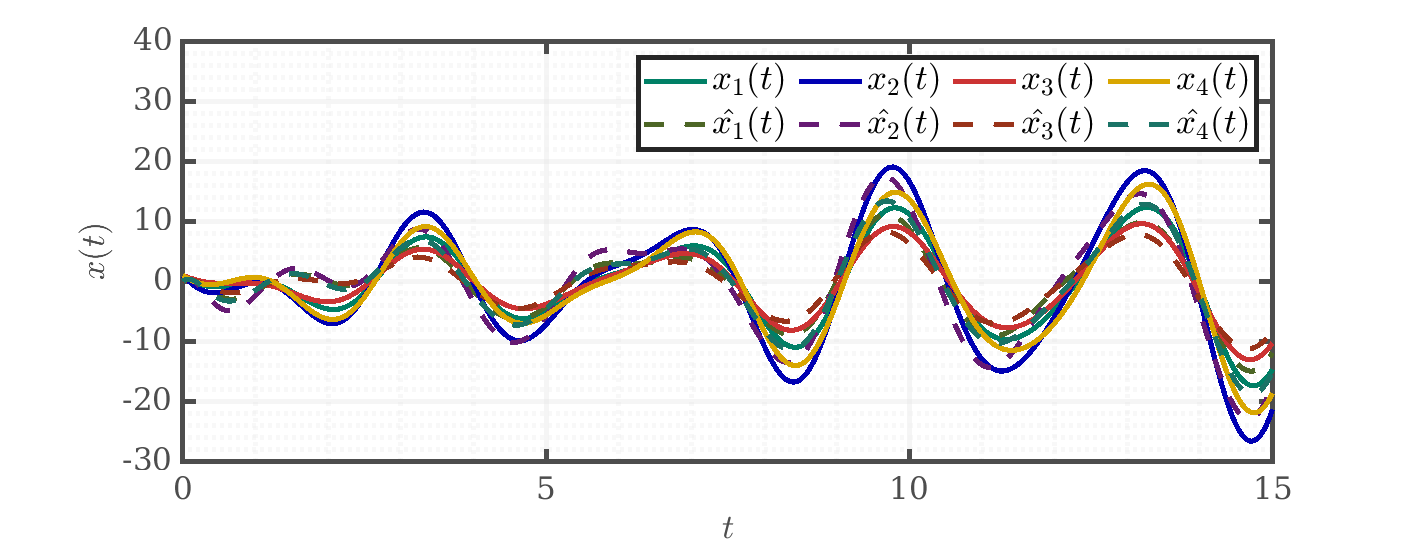
\includegraphics[width=\figwidth]{../../report/images/task2/x_compare_1.png}
	\caption{Сравнение $x(t)$ и $\hat{x}(t)$ для набора 1: $(Q_0, R_0)$}
\end{figure}

\begin{figure}[H]
	\centering
	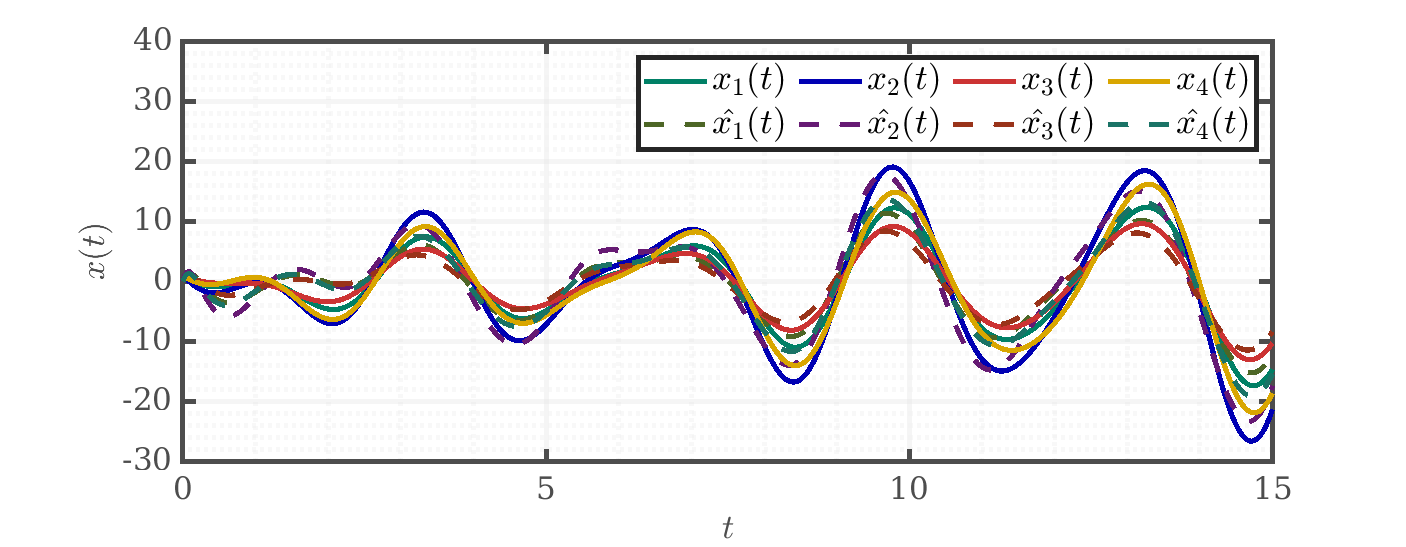
\includegraphics[width=\figwidth]{../../report/images/task2/x_compare_2.png}
	\caption{Сравнение $x(t)$ и $\hat{x}(t)$ для набора 2: $(\alpha Q_0, R_0)$}
\end{figure}

\begin{figure}[H]
	\centering
	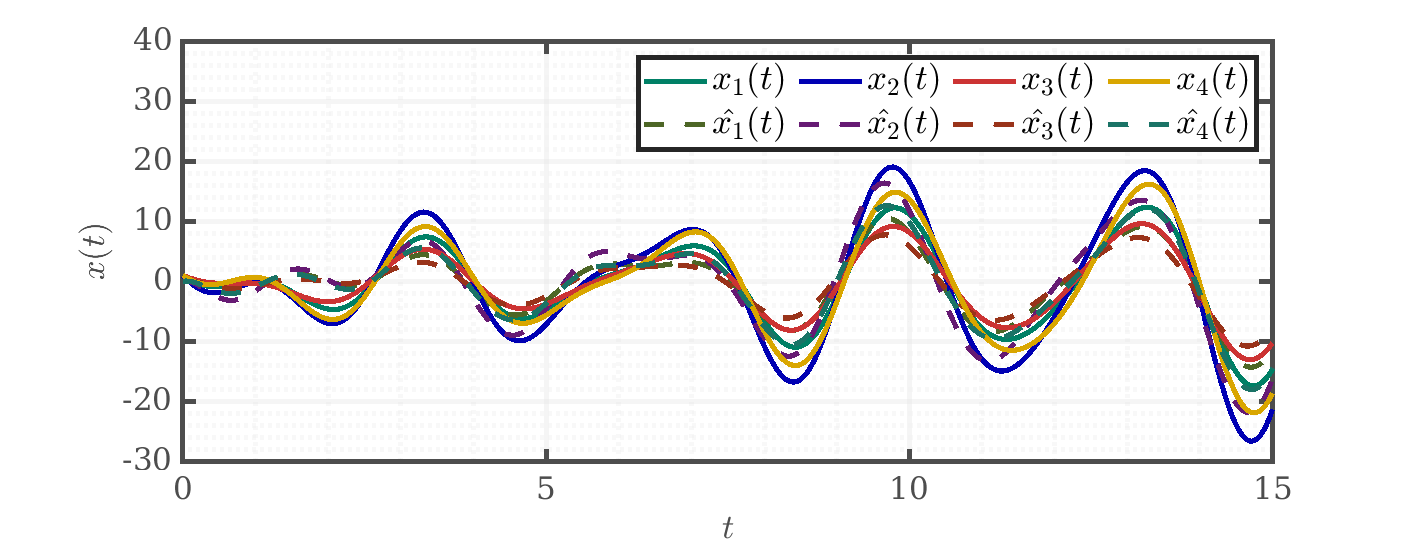
\includegraphics[width=\figwidth]{../../report/images/task2/x_compare_3.png}
	\caption{Сравнение $x(t)$ и $\hat{x}(t)$ для набора 3: $(Q_0, \alpha R_0)$}
\end{figure}

\begin{figure}[H]
	\centering
	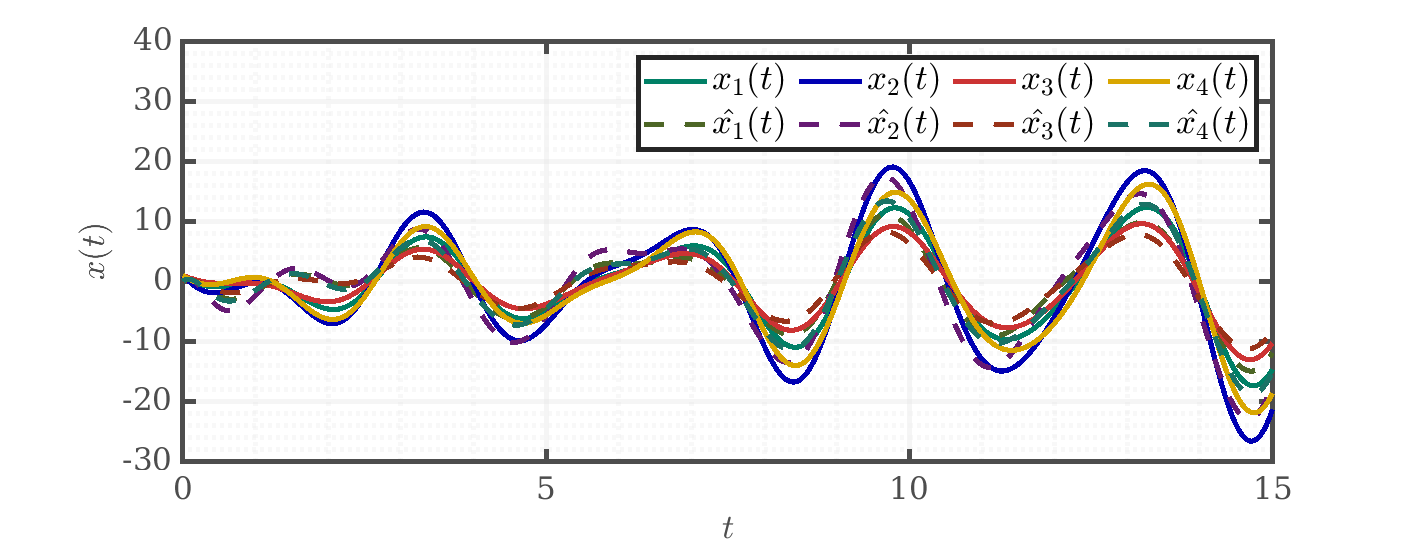
\includegraphics[width=\figwidth]{../../report/images/task2/x_compare_4.png}
	\caption{Сравнение $x(t)$ и $\hat{x}(t)$ для набора 4: $(\alpha Q_0, \alpha R_0)$}
\end{figure}	
	
	
	
\subsection{Выводы}

В ходе задания исследована система на наблюдаемость. Поскольку $\text{rank}(\mathcal{O}) = n$, система полностью наблюдаема, что позволило синтезировать устойчивый наблюдатель LQE.

Для четырёх наборов $(Q, R)$ вычислены матрицы коррекции $L$ и проведено моделирование. Установлено, что увеличение $Q$ усиливает $L$, уменьшая ошибку оценивания; увеличение $R$ ослабляет $L$, увеличивая ошибку. Одновременное масштабирование $Q$ и $R$ не меняет $L$.

Максимальная невязка не превысила значение $8$ по модулю, что подтверждает корректность синтеза. 

	
	\newpage
\section{Синтез LQG}


В соответствии с вариантом необходимо рассмотреть систему:

\[
\begin{cases}
	\dot{x} = Ax + Bu + f, \\
	y = Cx + Du + \xi,
\end{cases}
\qquad
x(0) = \begin{bmatrix} 1 & 1 & 1 & 1 \end{bmatrix}^T,
\]

где $f(t)$ и $\xi(t)$ --- гауссовские белые шумы (вариант нечётный).

Матрицы системы:

\[
A = \begin{bmatrix}
	5 & -9 & -7 & 1 \\
	-9 & 5 & -1 & 7 \\
	-7 & -1 & 5 & 9 \\
	1 & 7 & 9 & 5
\end{bmatrix}, \quad
B = \begin{bmatrix}
	3 & 0 \\
	3 & 0 \\
	1 & 0 \\
	3 & 0
\end{bmatrix}, \quad
C = \begin{bmatrix}
	2 & -2 & 2 & 2 \\
	-2 & 4 & 2 & 4
\end{bmatrix}, \quad
D = \begin{bmatrix}
	0 & 4 \\
	0 & 1
\end{bmatrix}.
\]

Требуется:

\begin{enumerate}
	\item Проверить систему на стабилизируемость и обнаруживаемость.
	
	\item Построить схему моделирования системы, замкнутой регулятором, состоящим из наблюдателя состояния и закона управления $u = K\hat{x}$.
	
	\item Задаться значениями пар матриц $(Q_K, R_K)$ для регулятора и $(Q_L, R_L)$ для наблюдателя.
	
	\item Синтезировать матрицу регулятора $K$ и наблюдателя $L$, решив уравнения Риккати:
	\[
	A^T P + P A + Q_K - P B R_K^{-1} B^T P = 0, \quad K = -R_K^{-1} B^T P;
	\]
	\[
	A P + P A^T + Q_L - P C^T R_L^{-1} C P = 0, \quad L = -P C^T R_L^{-1}.
	\]
	
	\item Выполнить моделирование с $\hat{x}(0)=0$, построить графики $u(t)$, $x(t)$, $\hat{x}(t)$ и ошибки $e(t)=x(t)-\hat{x}(t)$.
	
	\item Сделать выводы.
\end{enumerate}
	
\hrule \newpage

\subsection{Анализ стабилизируемости и обнаруживаемости}
	

Для проверки управляемости системы $(A, B)$ построена матрица управляемости:

\[
\mathcal{C} = \begin{bmatrix}
	B & AB & A^2B & A^3B
\end{bmatrix}
\]

Подставляя числовые значения матриц:

\[
\mathcal{C} = 
\begin{bmatrix}
	3 & 0 & -16 & 0 & -160 & 0 & -9088 & 0 \\
	3 & 0 & 8 & 0 & 512 & 0 & 5888 & 0 \\
	1 & 0 & 8 & 0 & 576 & 0 & 6656 & 0 \\
	3 & 0 & 48 & 0 & 352 & 0 & 10368 & 0
\end{bmatrix}
\]

\[
\text{rank}(\mathcal{C}) = 4 \qquad \text{rank}(A) = 4
\]

Так как $\text{rank}(\mathcal{C}) = \text{rank}(A)$, система является полностью управляемой. Следовательно, система \textit{стабилизируема}.

Для проверки наблюдаемости системы $(A, C)$ построена матрица наблюдаемости:

\[
\mathcal{O} = \begin{bmatrix}
	C \\ CA \\ CA^2 \\ CA^3
\end{bmatrix}
=
\begin{bmatrix}
	2 & -2 & 2 & 2 \\
	-2 & 4 & 2 & 4 \\
	16 & -16 & 16 & 16 \\
	-56 & 64 & 56 & 64 \\
	128 & -128 & 128 & 128 \\
	-1184 & 1216 & 1184 & 1216 \\
	1024 & -1024 & 1024 & 1024 \\
	-23936 & 24064 & 23936 & 24064
\end{bmatrix}
\]

\[
\text{rank}(\mathcal{O}) = 3 \qquad \text{rank}(A) = 4
\]

Так как $\text{rank}(\mathcal{O}) < \text{rank}(A)$, система не является полностью наблюдаемой. Перейду в жорданов базис (листинг~\ref{lst:jordan3}), чтобы выделить ненаблюдаемые моды.


В жордановом базисе матрицы системы имеют вид:

\[
J = V^{-1}AV = 
\begin{bmatrix}
	8 & 0 & 0 & 0 \\
	0 & -12 & 0 & 0 \\
	0 & 0 & 4 & 0 \\
	0 & 0 & 0 & 20
\end{bmatrix} \qquad
\tilde{C} = CV = 
\begin{bmatrix}
	8 & 0 & 0 & 0 \\
	0 & 0 & 4 & 12
\end{bmatrix}
\]


Ненаблюдаемой является вторая мода, которой соответствует собственное число $\lambda_2 = -12$. Так как $\Re(\lambda_2) = -12 < 0$, ненаблюдаемая мода устойчива. Значит система \textit{обнаруживаема}.
	
	
\subsection{Структурная схема системы}

Построю схему моделирования системы, замкнутой LQG-регулятором. Регулятор состоит из наблюдателя состояния и закона управления по оценке.

Объект управления описывается уравнениями:

\[
\begin{cases}
	\dot{x} = Ax + Bu + f \\
	y = Cx + Du + \xi
\end{cases}
\]

где $f(t)$ и $\xi(t)$ --- гауссовские белые шумы.

Наблюдатель состояния имеет структуру:

\[
\dot{\hat{x}} = A\hat{x} + Bu + L(y - C\hat{x} - Du), \qquad \hat{x}(0) =\begin{bmatrix} 0 & 0 & 0 & 0 \end{bmatrix}^T
\]

Закон управления формируется по оценке состояния:

\[
u = -K\hat{x}
\]

\begin{figure}[H]
	\centering
	
\includegraphics[width=1\textwidth]{../../report/images/task3/closed_observer.png}
	\caption{Схема моделирования системы с LQG-регулятором}
\end{figure}


\subsection{Выбор весовых матриц}

Для синтеза LQG-регулятора необходимо задаться весовыми матрицами для регулятора и наблюдателя.

\[
Q_K = I_4 =
\begin{bmatrix}
	1 & 0 & 0 & 0 \\
	0 & 1 & 0 & 0 \\
	0 & 0 & 1 & 0 \\
	0 & 0 & 0 & 1
\end{bmatrix} \qquad
R_K = I_2 =
\begin{bmatrix}
	1 & 0 \\
	0 & 1
\end{bmatrix}
\]

\[
Q_L = I_4 =
\begin{bmatrix}
	1 & 0 & 0 & 0 \\
	0 & 1 & 0 & 0 \\
	0 & 0 & 1 & 0 \\
	0 & 0 & 0 & 1
\end{bmatrix} \qquad
R_L = I_2 =
\begin{bmatrix}
	1 & 0 \\
	0 & 1
\end{bmatrix}
\]

	
\subsection{Синтез матрицы регулятора $K$}

Матрица $K$ находится из решения алгебраического уравнения Риккати (листинг~\ref{lst:K3}):

\[
A^T P + P A - P B R_K^{-1} B^T P + Q_K = 0
\]

Решение $P$ --- симметричная положительно определённая матрица:

\[
P = 
\begin{bmatrix}
	145.7888 & -185.6883 & 43.6764 & 3.7452 \\
	-185.6883 & 240.9213 & -63.8347 & -8.6586 \\
	43.6764 & -63.8347 & 30.1969 & 10.0473 \\
	3.7452 & -8.6586 & 10.0473 & 5.2207
\end{bmatrix}
\]

Матрица коэффициентов регулятора:

\[
K = -R_K^{-1} B^T P =
\begin{bmatrix}
	-64.7866 & 75.8884 & -0.1361 & 10.9694 \\
	0 & 0 & 0 & 0
\end{bmatrix}
\]
	
\subsection{Синтез матрицы наблюдателя $L$}

Матрица $L$ находится из решения алгебраического уравнения Риккати (листинг~\ref{lst:L3}):

\[
A P + P A^T - P C^T R_L^{-1} C P + Q_L = 0
\]

Решение $P$ --- симметричная положительно определённая матрица:

\[
P = 
\begin{bmatrix}
	3.6811 & 0.3883 & -3.1308 & 0.8969 \\
	0.3883 & 0.8369 & -0.8969 & 0.2866 \\
	-3.1308 & -0.8969 & 3.6811 & -0.3883 \\
	0.8969 & 0.2866 & -0.3883 & 0.8369
\end{bmatrix}
\]

Матрица коррекции наблюдателя:

\[
L = -P C^T R_L^{-1} =
\begin{bmatrix}
	2.1180 & -8.4830 \\
	-2.1180 & 1.9238 \\
	2.1180 & 8.4830 \\
	2.1180 & 1.9238
\end{bmatrix}
\]	
	
	

\subsection{Моделирование}

Возьму начальные условия объекта:
\(x(0) = \begin{bmatrix} 1 & 1 & 1 & 1 \end{bmatrix}^T\)

и начальные условия наблюдателя:

\(\hat{x}(0) = \begin{bmatrix} 0 & 0 & 0 & 0 \end{bmatrix}^T\)

Возмущения заданы в виде гауссовских белых шумов с параметрами:
\[
f(t) \sim \mathcal{N}(0, 0.1), \qquad \xi(t) \sim \mathcal{N}(0, 0.01)
\]
где $f(t)$ --- вектор размером $4 \times 1$, $\xi(t)$ --- скаляр.

Результаты моделирования замкнутой системы с LQG-регулятором представлены на рисунках \ref{fig:lqg_e}--\ref{fig:lqg_u}.

На рисунке \ref{fig:lqg_e} приведены графики ошибки оценивания $e(t) = x(t) - \hat{x}(t)$.

\begin{figure}[H]
	\centering
	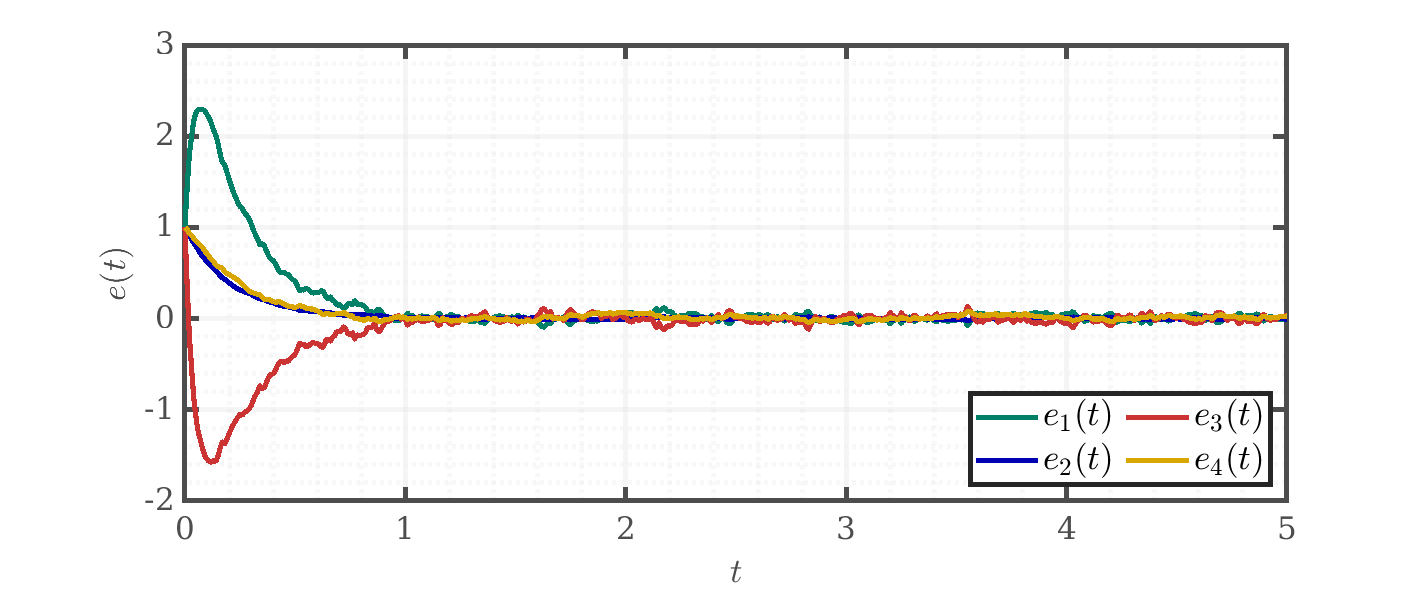
\includegraphics[width=\figwidth]{../../report/images/task3/e.png}
	\caption{Невязка $e(t) = x(t) - \hat{x}(t)$}
	\label{fig:lqg_e}
\end{figure}

На рисунке \ref{fig:lqg_x} представлено сравнение истинного состояния $x(t)$ и его оценки $\hat{x}(t)$.

\begin{figure}[H]
	\centering
	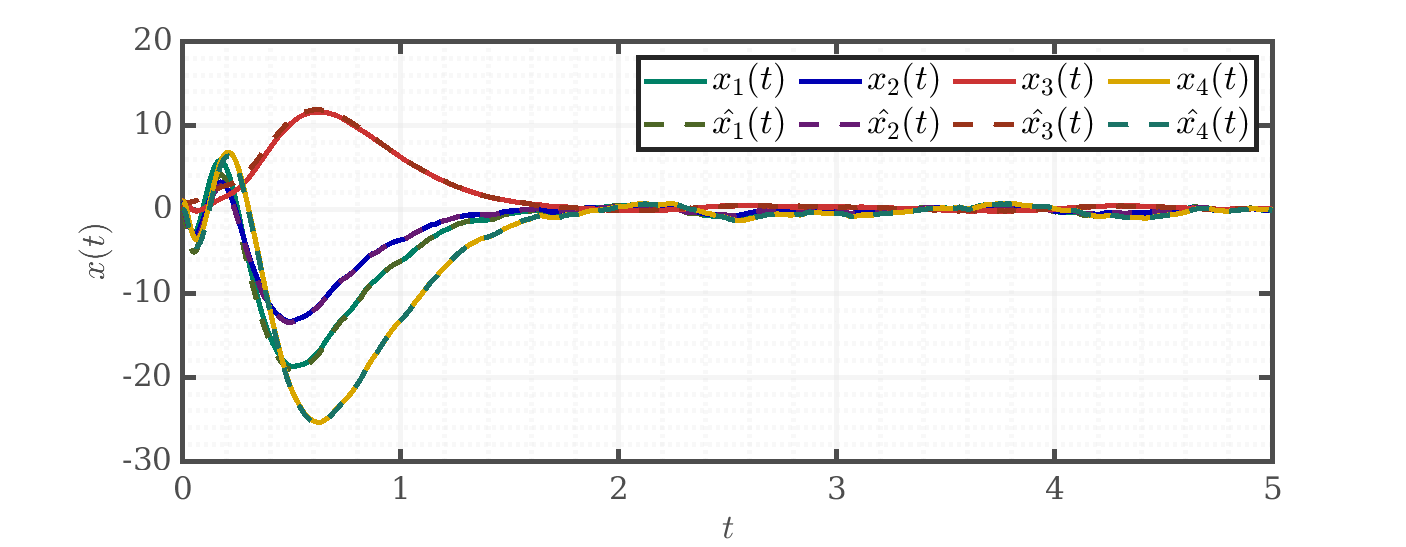
\includegraphics[width=\figwidth]{../../report/images/task3/x.png}
	\caption{Сравнение $x(t)$ и $\hat{x}(t)$}
	\label{fig:lqg_x}
\end{figure}

На рисунке \ref{fig:lqg_u} показан график управления $u(t)$, формируемого регулятором.

\begin{figure}[H]
	\centering
	
\includegraphics[width=\figwidth]{../../report/images/task3/u.png}
	\caption{Управление $u(t)$}
	\label{fig:lqg_u}
\end{figure}

\subsection{Выводы}

Система является стабилизируемой и обнаруживаемой, что позволило синтезировать устойчивый LQG-регулятор.

Регулятор по выходу, состоящий из LQR и наблюдателя, обеспечивает асимптотическую устойчивость замкнутой системы и минимизирует влияние случайных возмущений. Полная компенсация шумов $f(t)$ и $\xi(t)$ невозможна в силу их случайной природы, поэтому на $x(t)$, $y(t)$ и $u(t)$ сохраняются малые колебания.

Наблюдатель обеспечивает сходимость $\hat{x}(t)$ к $x(t)$ с ошибкой, ограниченной уровнем шумов. Управление $u(t)$ остаётся ограниченным и эффективно стабилизирует систему.


	
\newpage

\section{Вывод}

В ходе работы синтезированы LQR-регулятор, LQE-наблюдатель и LQG-регулятор.

Для LQR показано, что увеличение $Q$ ускоряет переходные процессы, увеличение $R$ ослабляет управление, одновременное масштабирование $Q$ и $R$ не меняет $K$.

Для LQE установлено, что увеличение $Q$ усиливает $L$ и уменьшает ошибку оценивания, увеличение $R$ даёт обратный эффект.

Для LQG система стабилизируема и обнаруживаема. Регулятор обеспечивает устойчивость и минимизирует влияние шумов, однако полностью компенсировать их невозможно. Оценка состояния $\hat{x}(t)$ сходится к $x(t)$, управление $u(t)$ остаётся ограниченным.	
	
	
	
	
	
	
	
	
	
\newpage
\section{Приложение}

\subsection*{Задание 1}

\begin{lstlisting}[caption={Инициализация}]
A = [8  1  11, 4  0  4 , -4 -3  -7];
B = [-1 -3 3]';
x0 = [1 1 1]';

Q0 = eye(3);
R0 = 1;
alpha = 5;

Q_set = {Q0, alpha*Q0, Q0, alpha*Q0};
R_set = {R0, R0, alpha*R0, alpha*R0};
	
K_cell = cell(1,4);
P_cell = cell(1,4);
Jmin_vec = zeros(1,4);
\end{lstlisting}

\begin{lstlisting}[caption={Вещественная Жорданова форма}, label={lst:jordan1}]
[P, J] = jordan(sym(A)); P = double(P); J = double(J);
[P_real, J_real] = cdf2rdf(P, J)
B_tilde = inv(P_real) * B
\end{lstlisting}


\begin{lstlisting}[caption={Расчет \(K\), \(P\), \(J\)}, label={lst:LQR1}]
for i = 1:4
	Q = Q_set{i};
	R = R_set{i};
	
	[K, P, ~] = lqr(A, B, Q, R)
	
	Jmin = x0' * P * x0;
	
	P_cell{i} = P;
	K_cell{i} = K;
	Jmin_vec(i) = Jmin;
end
\end{lstlisting}	
	
	\newpage
\subsection*{Задание 2}

\begin{lstlisting}[caption={Инициализация}]
A = [-40  16   9   7;
	-64  25  14  12;
	-26  11   7   3;
	-48  18  14   8];

C = [-3  2  -2  1];
x0 = [1 1 1 1]';
x0_hat = [0 0 0 0]';

Q0 = eye(4);   
R0 = 1;       
alpha = 5;

Q_set = {Q0, alpha*Q0, Q0, alpha*Q0};
R_set = {R0, R0, alpha*R0, alpha*R0};
L_cell = cell(1,4);
\end{lstlisting}

\begin{lstlisting}[caption={Анализ стабилизируемости}, label={lst:obsv}]
O = obsv(A, C)
rank_O = rank(O) == rank(A)
\end{lstlisting}
	
	
\begin{lstlisting}[caption={Расчет \(L\), \(P\)}, label={lst:LQE2}]
for i = 1:4
	Q = Q_set{i};
	R = R_set{i};
	[P, ~, ~] = care(A', C', Q, R)
	L_cell{i} = P * C' * inv(R);
	L_cell{i}
end
\end{lstlisting}

\newpage
\subsection*{Задание 1}

\begin{lstlisting}[caption={Инициализация}]
A = [5 -9 -7 1;
	-9 5 -1 7;
	-7 -1 5 9;
	1 7 9 5];

B = [3 0;
	3 0;
	1 0;
	3 0];
C = [2 -2 2 2; 
	-2 4 2 4];

D = [0 4;
	0 1];

x0=[1 1 1 1]';
x0_hat=[0 0 0 0]';

QK = eye(4); RK = eye(2);
QL = eye(4); RL = eye(2);
\end{lstlisting}

\begin{lstlisting}[caption={Матрицы в Жордановом базисе}, label={lst:jordan3}]
[V, J] = jordan(sym(A));
J = double(J); V = double(V);

C_tilde = C * V
J = V \ A * V
\end{lstlisting}

\begin{lstlisting}[caption={Синтез матрицы регулятора \(K\)}, label={lst:K3}]
[K, PK, ~] = lqr(A, B, QK, RK)
\end{lstlisting}

\begin{lstlisting}[caption={Синтез матрицы наблюдателя \(L\)}, label={lst:L3}]
[PL, ~, ~] = care(A', C', QL, RL);
L = PL * C' * inv(RL);
\end{lstlisting}
	

	
\end{document}